% =============================================================================
%  Rapport d'ingénierie des données — Projet 4 : supervision temps réel de bornes de recharge (FR)
%  Compilation : latexmk -xelatex rapport-fr.tex
% =============================================================================
\documentclass[11pt, a4paper, oneside, headings=normal, numbers=noenddot, DIV=12]{scrartcl}
\usepackage[french]{babel}
\usepackage{report-style}
\graphicspath{{../livraison/figures/fr/}}
\sisetup{locale=FR, group-minimum-digits=4}

\newcommand{\ReportAuthor}{LUMU BAMANA MANASSE}
\newcommand{\ReportAuthorRole}{Data engineer}
\newcommand{\ReportShortTitle}{Supervision des bornes · Rapport d'ingénierie des données}
\newcommand{\ReportFooter}{Octobre 2026 · v1.0.0}
\newcommand{\ReportKicker}{Rapport d'ingénierie des données · Projet 4}
\newcommand{\ReportTitle}{Une panne détectée\\en quelques secondes}
\newcommand{\ReportSubtitle}{Supervision temps réel de bornes de recharge :\\Kafka, Spark Structured Streaming, Iceberg, Grafana et Terraform}
\newcommand{\ReportMeta}{%
  \begin{tabularx}{\linewidth}{@{}>{\bfseries}l@{\hspace{1em}}Y@{}}
  Date & Octobre 2026 \\
  Version & 1.0.0 (livrée et recettée) \\
  Client & Lumio Recharge (entreprise fictive) · Mission LUM-2026-002 \\
  Dépôt GitHub & \url{https://github.com/MediJr/ev-charging-realtime-streaming} \\
  Langue & Français · \textit{English version available in the repository}
  \end{tabularx}}
\newcommand{\ReportScenario}{Scénario fictif, bornes simulées, données carbone réelles : l'entreprise cliente et ses interlocuteurs sont inventés
  pour simuler une mission professionnelle complète ; les mesures des bornes sont produites par un simulateur. L'intensité carbone est la donnée
  éCO2mix temps réel de RTE (Open Data Réseaux Énergies, Licence Ouverte). Ce projet n'est ni commandé, ni validé, ni affilié à RTE.}
\hypersetup{pdftitle={Savoir en quelques secondes qu'une borne va mal : rapport d'ingénierie des données}, pdfauthor={Lumu Bamana Manasse},
  pdfsubject={Streaming Kafka, Spark, Iceberg, Grafana, Terraform, projet de portfolio}, pdflang={fr-FR}}

\begin{document}
\sloppy
\MakeTitlePage

% =============================================================================
\section*{Fiche du document}
\addcontentsline{toc}{section}{Fiche du document}

\begin{tabularx}{\linewidth}{@{}>{\bfseries\sffamily}L{4.2cm}Y@{}}
\toprule
Projet & Projet 4 du portfolio : streaming, lakehouse et infrastructure en code \\
Mission & LUM-2026-002 : « Savoir en quelques secondes qu'une borne ne va pas bien » \\
Client & Lumio Recharge, opérateur de 1\,200 bornes (fictif), à l'attention de Sophie Bernard et Karim Haddad \\
Auteur & Lumu Bamana Manasse, data engineer \\
Période de réalisation & Octobre 2026 \\
Données & 200 bornes simulées (une mesure toutes les 5~s) ; intensité carbone réelle de RTE \\
Statut & \pill{good}{LIVRÉ} \pill{good}{RECETTÉ} \\
Code source & \url{https://github.com/MediJr/ev-charging-realtime-streaming} \\
\bottomrule
\end{tabularx}

\subsection*{Historique des versions}
\begin{tabularx}{\linewidth}{@{}l l Y@{}}
\toprule
\textbf{Version} & \textbf{Date} & \textbf{Objet} \\
\midrule
0.1 & 26/10/2026 & Cadrage : brief, compte rendu, cahier des charges \\
0.5 & 26/10/2026 & Plateforme de streaming, lakehouse, supervision, Terraform \\
0.9 & 27/10/2026 & Endurance de 31~h : deux défauts corrigés \\
1.0.0 & 27/10/2026 & Recette (panne, charge, rattrapage), rapport final (français et anglais) \\
\bottomrule
\end{tabularx}

\subsection*{Guide de lecture}
\begin{tabularx}{\linewidth}{@{}>{\bfseries}L{4.2cm}Y@{}}
Direction des opérations & \hyperref[sec:resume]{1. Résumé exécutif} et \hyperref[sec:resultats]{10. Résultats} \\
DSI (passage au cloud) & 4. Architecture, 8. Infrastructure GCP, 12. Feuille de route \\
Ingénieur reprenant le projet & 5. Traitement, 6. Lakehouse, 9. Recette, 11. Retour d'expérience \\
\end{tabularx}

\begingroup
\addtokomafont{sectionentry}{\color{primary}}
\setcounter{tocdepth}{2}
\tableofcontents
\endgroup
\clearpage

% =============================================================================
\section{Résumé exécutif}\label{sec:resume}

\textbf{Le besoin.} Lumio Recharge apprend qu'une borne est en panne quand un client appelle, parfois des heures plus tard. Ses bornes envoient
pourtant leur puissance toutes les 5 secondes. L'exploitation veut être alertée \textbf{en moins de 30 secondes}, voir le \textbf{CO\textsubscript{2}
de chaque recharge en direct}, et superviser le parc sur un écran. La DSI prévoit Google Cloud l'an prochain.

\textbf{La solution.} Une plateforme de \textbf{streaming} démarrée par un seul \texttt{docker compose up}. Les mesures passent par un journal
d'événements compatible \textbf{Kafka} (Redpanda), sont traitées en \textbf{temps d'événement} par \textbf{Spark Structured Streaming}
(watermark, dédoublonnage, état par borne), conservées dans un \textbf{lakehouse Apache Iceberg}, enrichies de l'intensité carbone
\textbf{réelle} de RTE, et affichées dans \textbf{Grafana}. L'infrastructure Google Cloud cible est décrite en \textbf{Terraform}.

\kpirow{27 / 27}{anomalies\\détectées}{11,6 s}{délai de détection\\au 95\textsuperscript{e} centile}{0}{fausse\\alerte}{0}{message perdu ou doublé\\après arrêt brutal}
\kpirow{83\,292}{messages rapprochés\\un par un}{8,4 s}{pour rattraper\\3\,654 messages}{≈ 1\,440}{messages/s\\(capacité mesurée)}{22}{tests, dont 5 Spark\\de bout en bout}

\begin{keybox}[Ce qu'il faut retenir]
\begin{itemize}[leftmargin=1.2em]
  \item \textbf{Q1 · Délai :} les 27 anomalies injectées sont détectées en 5,9~s (médiane) et 11,6~s (95\textsuperscript{e} centile). Objectif : 30~s.
  \item \textbf{Q2 · Anomalies :} borne muette, surpuissance, borne bloquée, chacune ouverte puis résolue, sans déluge d'alertes.
  \item \textbf{Q3 · CO\textsubscript{2} :} 186 recharges, 4,8~MWh, 211~kg de CO\textsubscript{2} à l'intensité RTE réelle de la soirée (44~g/kWh).
  \item \textbf{Q4 · Robustesse :} Spark tué en plein flux, reprise sans perte ni doublon. Capacité d'environ 1\,440 messages/s, soit
        quelque 7\,000 bornes : six fois le parc actuel.
\end{itemize}
\end{keybox}

\textbf{Trois défauts ont été trouvés en faisant tourner la plateforme pour de vrai} (31~h d'endurance, panne, surcharge), corrigés et
couverts par des tests : une colonne de dates vide refusée par Arrow, des identifiants de mesure répétés après un redémarrage, et des bornes
muettes manquées pendant un rattrapage.

% =============================================================================
\section{Contexte et cadrage}

\begin{table}[H]
\centering\small
\begin{tabularx}{\linewidth}{@{}L{5.8cm} Y@{}}
\toprule
\textbf{Demande du client} & \textbf{Conséquence technique} \\
\midrule
« Détecter en quelques secondes » & Traitement \textbf{continu} (streaming), pas par lots \\
« Une borne qui ne répond plus » & Détecter une \textbf{absence} d'événement : état par borne et délai \\
Réseau 4G qui retarde ou double les messages & \textbf{Temps d'événement}, watermark, dédoublonnage \\
« Sans tout réécrire sur Google Cloud » & Formats ouverts (Iceberg), API Kafka, infrastructure en \textbf{Terraform} \\
Une panne ne doit rien perdre ni doubler & Points de reprise (checkpoints), écritures idempotentes \\
\bottomrule
\end{tabularx}
\caption{De la demande aux exigences techniques}
\end{table}

\begin{table}[H]
\centering\small
\begin{tabularx}{\linewidth}{@{}L{3.3cm} Y L{2.3cm}@{}}
\toprule
\textbf{Anomalie} & \textbf{Règle (cadrage)} & \textbf{Gravité} \\
\midrule
Borne muette & Aucun message depuis plus de 60~s & critique \\
Surpuissance & Puissance supérieure à 110~\% de la puissance nominale & haute \\
Borne bloquée & Session ouverte à 0~kW depuis plus de 2~minutes & moyenne \\
\bottomrule
\end{tabularx}
\caption{Les trois anomalies et leurs règles}
\end{table}

% =============================================================================
\section{Données}

\textbf{Mesures des bornes (simulées).} 200 bornes sur 12 sites, deux tiers en 22~kW et un tiers en 50~kW, une mesure toutes les 5~s :
puissance, énergie de la session, état, session en cours. Le simulateur injecte \textbf{volontairement} des défauts, et publie chaque injection
dans un topic de \textbf{vérité terrain} (\texttt{sim.injections}) qui permet de vérifier chaque détection.

\begin{table}[H]
\centering\small
\begin{tabularx}{\linewidth}{@{}L{4.4cm} L{3.2cm} Y@{}}
\toprule
\textbf{Défaut injecté} & \textbf{Fréquence} & \textbf{Ce qu'il éprouve} \\
\midrule
Borne muette, surpuissance, borne bloquée & ≈ 0,3 par borne et par heure & Les trois règles d'anomalie \\
Message en double & 1~\% & Dédoublonnage \\
Retard de 5 à 40~s & 1~\% & Temps d'événement \\
Retard de 3 à 5~min & 0,2~\% & Watermark : écarté et compté \\
\bottomrule
\end{tabularx}
\caption{Défauts injectés par le simulateur (ADR 005)}
\end{table}

\textbf{Intensité carbone (réelle).} Un collecteur lit toutes les 5 minutes l'API éCO2mix temps réel de RTE, la même source qu'au projet 2,
et publie chaque créneau de 15 minutes dans un topic \textbf{compacté} : seule la dernière valeur de chaque créneau est conservée.

% =============================================================================
\section{Architecture}

\begin{figure}[H]
\centering
\resizebox{\linewidth}{!}{%
\begin{tikzpicture}[
  font=\sffamily\small, node distance=0.6cm and 0.75cm,
  src/.style={draw=rule, fill=panel, rounded corners=2pt, minimum width=2.4cm, minimum height=1.1cm, align=center},
  stage/.style={draw=primary, fill=primary, text=white, rounded corners=3pt, minimum width=2.6cm, minimum height=1.3cm, align=center, font=\sffamily\small\bfseries},
  store/.style={cylinder, shape border rotate=90, aspect=0.18, draw=accent, fill=accent!8, minimum width=2.3cm, minimum height=1.3cm, align=center},
  arr/.style={-{Stealth[length=2.6mm]}, thick, color=ink2}]
  \node[src] (sim) {Simulateur\\\scriptsize 200 bornes};
  \node[src, below=0.5cm of sim] (rte) {API RTE\\\scriptsize CO\textsubscript{2} temps réel};
  \node[store, right=1.2cm of $(sim)!0.5!(rte)$] (rp) {\scriptsize Redpanda\\\scriptsize API Kafka};
  \node[stage, right=1.2cm of rp] (sp) {SPARK\\\scriptsize\mdseries temps d'événement\\\scriptsize\mdseries watermark · état};
  \node[store, right=1.6cm of sp, yshift=1.1cm] (ice) {\scriptsize Iceberg (S3)\\\scriptsize bronze·silver·gold};
  \node[store, right=1.6cm of sp, yshift=-1.1cm] (pg) {\scriptsize PostgreSQL\\\scriptsize diffusion};
  \node[src, right=0.9cm of pg] (gf) {Grafana\\\scriptsize 13 panneaux};
  \draw[arr] (sim) -- (rp); \draw[arr] (rte) -- (rp); \draw[arr] (rp) -- (sp);
  \draw[arr] (sp) -- (ice); \draw[arr] (sp) -- (pg); \draw[arr] (pg) -- (gf);
  \draw[arr, dashed] (sp.north) to[bend right=35] node[above, font=\scriptsize\sffamily, text=ink2]{charger.alerts} (rp.north);
\end{tikzpicture}}
\caption{De la borne à l'écran de supervision}
\end{figure}

\begin{table}[H]
\centering\small
\begin{tabularx}{\linewidth}{@{}L{3cm} L{3.6cm} Y@{}}
\toprule
\textbf{Rôle} & \textbf{Choix} & \textbf{Pourquoi (ADR)} \\
\midrule
Journal d'événements & Redpanda v25.3 & Protocole Kafka, un seul binaire, léger ; remplaçable par un Kafka managé (001) \\
Traitement & Spark 4.0 Structured Streaming & Temps d'événement, watermark, état tolérant aux pannes (001) \\
Lakehouse & Iceberg 1.10 sur S3, catalogue JDBC & Transactions, format ouvert lu par BigQuery (002) \\
Diffusion & PostgreSQL 17 & Rafraîchissement de l'écran en quelques millisecondes (003) \\
Supervision & Grafana 12, provisionné en code & Standard de l'observabilité (003) \\
Cloud & Terraform, fournisseur Google 8.8 & Infrastructure relue et versionnée avant d'exister (004) \\
\bottomrule
\end{tabularx}
\caption{Choix techniques}
\end{table}

% =============================================================================
\section{Traitement Spark}

Une seule application Spark exécute six requêtes, chacune avec son point de reprise :

\begin{table}[H]
\centering\small
\begin{tabularx}{\linewidth}{@{}L{2.2cm} L{1.6cm} Y L{3.4cm}@{}}
\toprule
\textbf{Requête} & \textbf{Rythme} & \textbf{Traitement} & \textbf{Destination} \\
\midrule
bronze & 30~s & Aucun : le message tel que reçu, avec sa position Kafka & Iceberg \\
silver & 30~s & Lecture du JSON, watermark de 2~min, dédoublonnage & Iceberg \\
monitor & 5~s & État par borne et règles d'anomalie & PostgreSQL, Kafka, Iceberg \\
minutes & 30~s & Énergie par borne et par minute close, CO\textsubscript{2} & PostgreSQL, Iceberg \\
grid\_co2 & 30~s & Intensité carbone RTE & PostgreSQL, Iceberg \\
injections & 30~s & Vérité terrain du simulateur & PostgreSQL \\
\bottomrule
\end{tabularx}
\caption{Les six requêtes en continu}
\end{table}

\subsection{Temps d'événement, watermark et dédoublonnage}
Une mesure est rangée selon l'heure \textbf{où la borne l'a produite}, pas selon l'heure où elle arrive. La \textbf{watermark} de 2~minutes
indique jusqu'où Spark attend les retardataires : au-delà, une mesure est écartée, et comptée dans le suivi des micro-lots. Le dédoublonnage
porte sur l'identifiant de la mesure, \texttt{event\_id}.

\subsection{L'état par borne et la détection d'une absence}
Les règles sont écrites en \textbf{Python pur} (\texttt{lumio\_stream.monitor}), testées sans Spark. Spark les appelle pour chaque borne avec ses
nouvelles mesures et l'état mémorisé (\texttt{applyInPandasWithState}). Une borne qui n'envoie plus rien n'appelle plus rien : c'est un
\textbf{délai de traitement} de 60~s, posé à chaque mesure reçue, qui déclenche l'alerte « borne muette ».

\begin{warnbox}[Limite découverte en recette : le rattrapage]
Quand Spark rattrape un retard, il traverse plusieurs minutes de temps d'événement en quelques secondes : le délai de traitement ne se
déclenche pas, et 3 bornes muettes ont été manquées. Un \textbf{filet de sécurité en temps d'événement} a été ajouté : un trou de plus de 60~s
entre deux mesures, constaté au retour de la borne, ouvre et ferme l'alerte. Elle arrive en retard, mais n'est \textbf{jamais perdue}.
\end{warnbox}

% =============================================================================
\section{Lakehouse Iceberg}

\begin{table}[H]
\centering\small
\begin{tabularx}{\linewidth}{@{}L{3.6cm} L{3.2cm} Y@{}}
\toprule
\textbf{Table} & \textbf{Grain} & \textbf{Contenu} \\
\midrule
bronze.telemetry\_raw & un message Kafka & Message brut, partition et position Kafka \\
silver.telemetry & une mesure & Champs typés, dédoublonnés \\
gold.charger\_minute & borne × minute & Énergie, CO\textsubscript{2} \\
gold.alerts & changement d'état & Alerte ouverte ou résolue, heures d'anomalie et de détection \\
\bottomrule
\end{tabularx}
\caption{Les tables du lakehouse (partitionnées par jour)}
\end{table}

\textbf{Exactement une fois.} Le puits Iceberg natif de Spark l'est par construction. Pour les écritures faites dans \texttt{foreachBatch},
qui ne garantit qu'« au moins une fois », chaque ajout est marqué du numéro de micro-lot dans l'instantané Iceberg : un lot rejoué après une panne
est ignoré. Les écritures de diffusion sont des UPSERT.

\textbf{Maintenance.} Le streaming écrit un petit fichier par micro-lot. Un script quotidien supprime les mesures brutes de plus de 90 jours,
compacte les petits fichiers et expire les anciens instantanés.

% =============================================================================
\section{Supervision}

L'écran Grafana (13 panneaux, provisionnés en code, accès anonyme en lecture seule) montre en premier les \textbf{alertes ouvertes} triées par
gravité, puis les bornes en ligne, la puissance du parc, l'intensité RTE, le délai de détection au 95\textsuperscript{e} centile, le débit, les
recharges en cours avec leur CO\textsubscript{2}, et la santé du flux (lignes écartées par la watermark). Un \texttt{StreamingQueryListener}
enregistre chaque micro-lot dans la base de diffusion.

% =============================================================================
\section{Infrastructure Google Cloud en Terraform}

\begin{table}[H]
\centering\small
\begin{tabularx}{\linewidth}{@{}L{4.2cm} Y@{}}
\toprule
\textbf{Ressource} & \textbf{Choix} \\
\midrule
Bucket du lakehouse & Région Paris, accès public interdit, versionnage, mesures brutes supprimées après 90 jours \\
BigQuery + BigLake & Dataset des tables gold ; connexion BigLake pour lire Iceberg sans copie \\
Comptes de service & Un par usage : le traitement écrit, la supervision lit seulement \\
Alerte de budget & 50, 90 et 100~\% d'un budget mensuel \\
\bottomrule
\end{tabularx}
\caption{Infrastructure décrite (ADR 004)}
\end{table}

\texttt{terraform fmt}, \texttt{init -backend=false} et \texttt{validate} passent, en local et dans l'intégration continue. Le \texttt{plan}
demande des identifiants GCP : il sera fait avec la DSI. Correspondance : SeaweedFS devient Cloud Storage, Spark local devient Dataproc
Serverless (même code), Redpanda devient Kafka managé (même protocole).

% =============================================================================
\section{Recette}

La recette a été passée sur une \textbf{plateforme vierge}, avec un arrêt brutal de Spark en plein flux, puis un test de charge.

\begin{table}[H]
\centering\small
\begin{tabularx}{\linewidth}{@{}l Y c@{}}
\toprule
\textbf{\#} & \textbf{Critère} & \textbf{Résultat} \\
\midrule
C1 & Démarrage avec \texttt{docker compose up} sur une plateforme vierge & \ok \\
C2 & Les trois anomalies injectées détectées (27 / 27, 0 fausse alerte) & \ok \\
C3 & Délai de détection < 30~s au 95\textsuperscript{e} centile (11,6~s) & \ok \\
C4 & Doublons comptés une fois, retardataires comptés à part & \ok \\
C5 & Arrêt brutal de Spark : ni perte, ni doublon & \ok \\
C6 & CO\textsubscript{2} calculé avec l'intensité RTE réelle & \ok \\
C7 & Terraform validé, tests verts & \ok \\
C8 & Aucun secret versionné & \ok \\
\bottomrule
\end{tabularx}
\caption{Critères d'acceptation : 8 sur 8}
\end{table}

\subsection{Rapprochement : chaque message est expliqué}

\begin{terminal}{spark/recette.py · messages arrivés avant 19:46:59}
\begin{lstlisting}[style=terminal]
messages bronze                :    83,292   (positions Kafka distinctes : 83,292)
identifiants distincts         :    82,484   -> doublons écartés : 808
mesures silver                 :    82,347   (identifiants distincts : 82,347)
identifiants absents de silver :       137
équation : 83,292 = 82,347 + 808 + 137  -> OK
message lu deux fois par Spark : 0
injections avant la coupure    : {'too_late': 164, 'late': 882, 'duplicate': 808}
absents de silver expliqués par un retard injecté de 3 à 5 min : 137 / 137
\end{lstlisting}
\end{terminal}

Les 808 doublons écartés sont exactement les 808 doublons injectés. Les 137 mesures absentes sont toutes des retards injectés au-delà de la
watermark. Aucun message Kafka n'a été lu deux fois, malgré l'arrêt brutal de Spark : le premier micro-lot après la relance porte le numéro 41,
juste après le 40 validé avant la panne, et rattrape 3\,654 messages en 8,4~s.

% =============================================================================
\section{Résultats}\label{sec:resultats}

\subsection*{Q1 · Délai de détection}
\begin{figure}[H]
\centering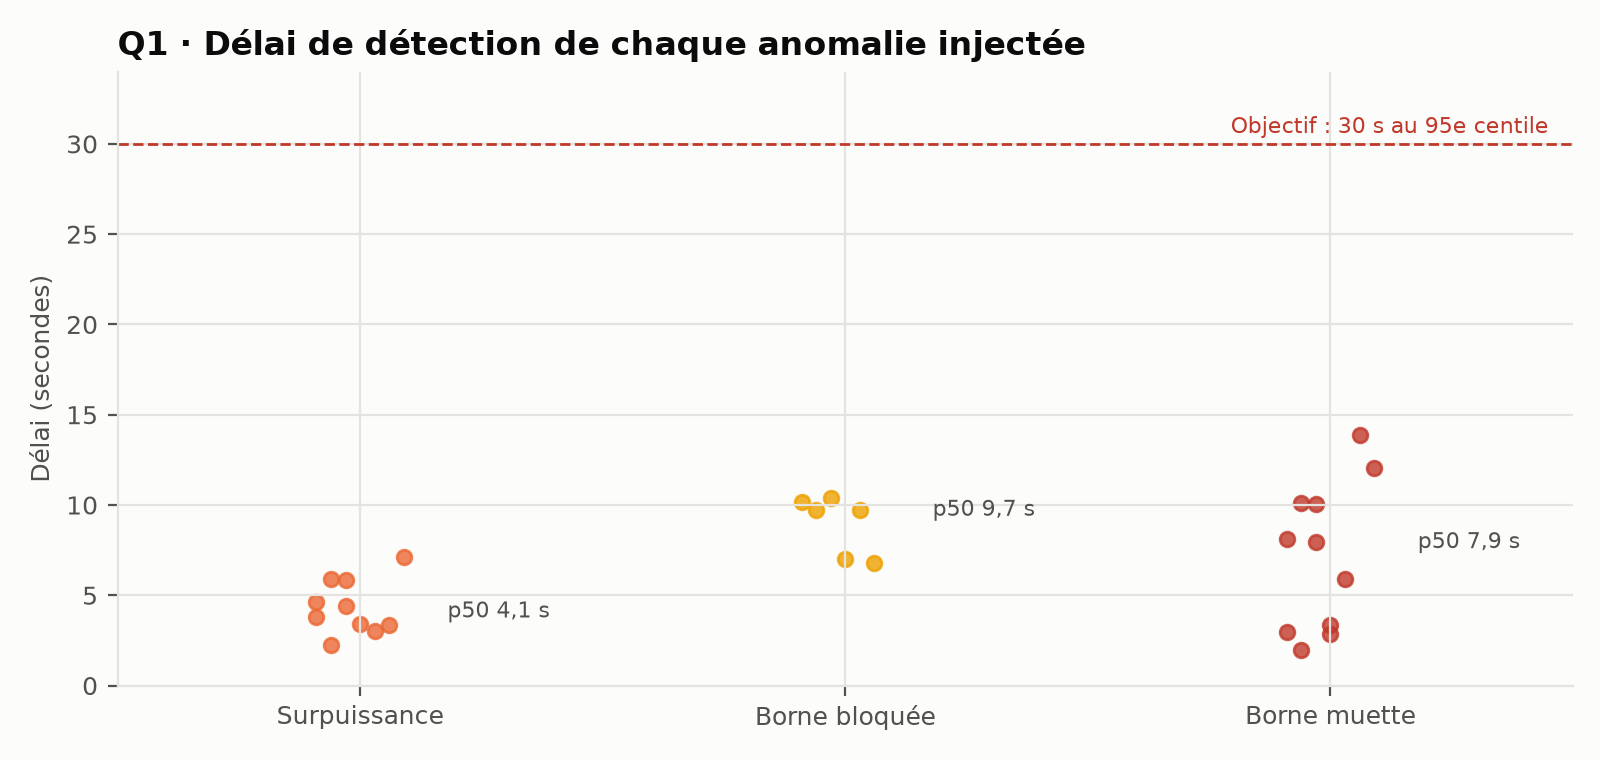
\includegraphics[width=0.86\linewidth]{q1_delai_detection.png}
\end{figure}
Les 27 anomalies injectées pendant la période nominale sont toutes détectées, sans fausse alerte : surpuissance en 4,1~s (médiane), borne
bloquée en 9,7~s, borne muette en 7,9~s. Le 95\textsuperscript{e} centile est de \textbf{11,6~s}, le maximum de 13,9~s.

\subsection*{Q2 · Alertes par site}
\begin{figure}[H]
\centering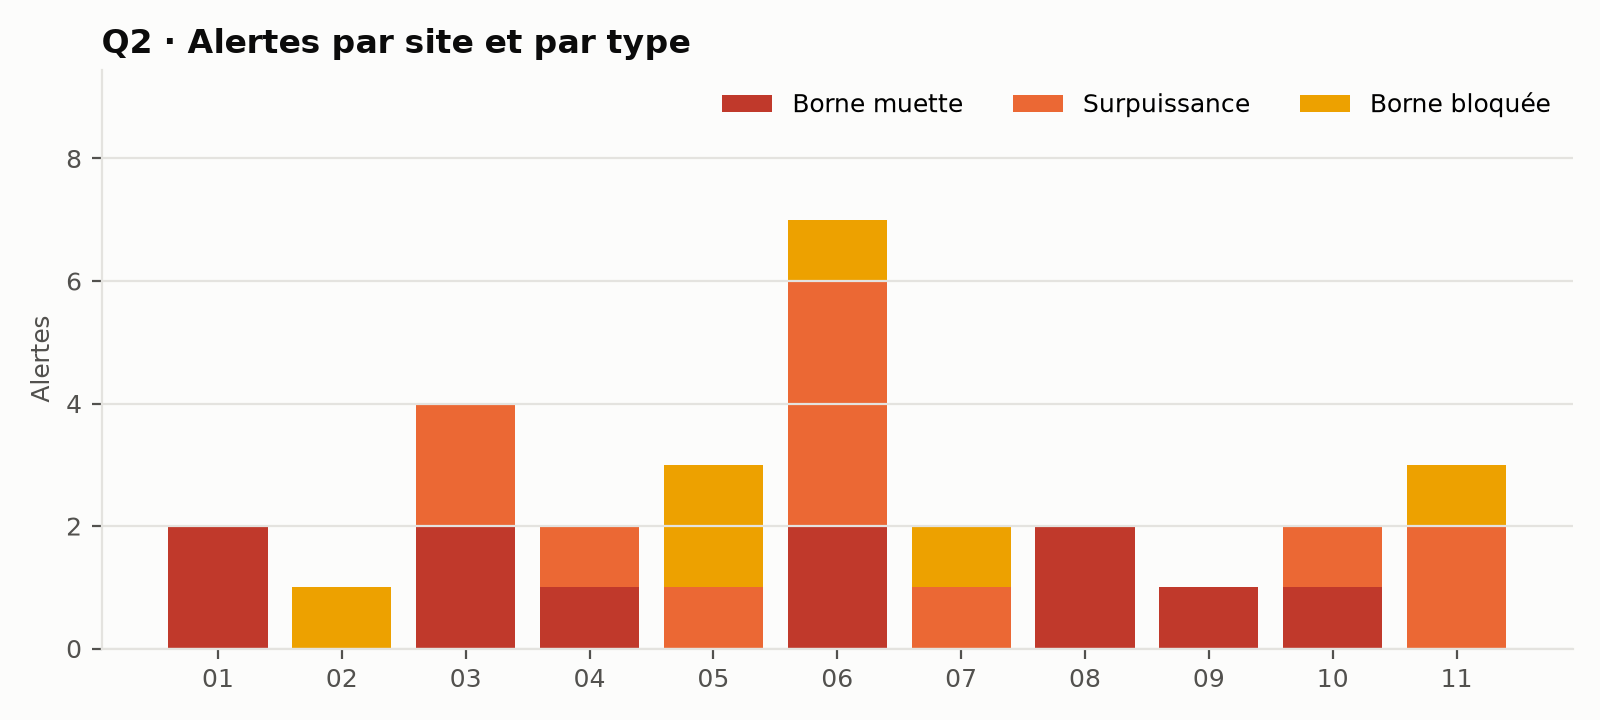
\includegraphics[width=0.86\linewidth]{q2_alertes_par_site.png}
\end{figure}

\subsection*{Q3 · CO\textsubscript{2} des recharges}
\begin{figure}[H]
\centering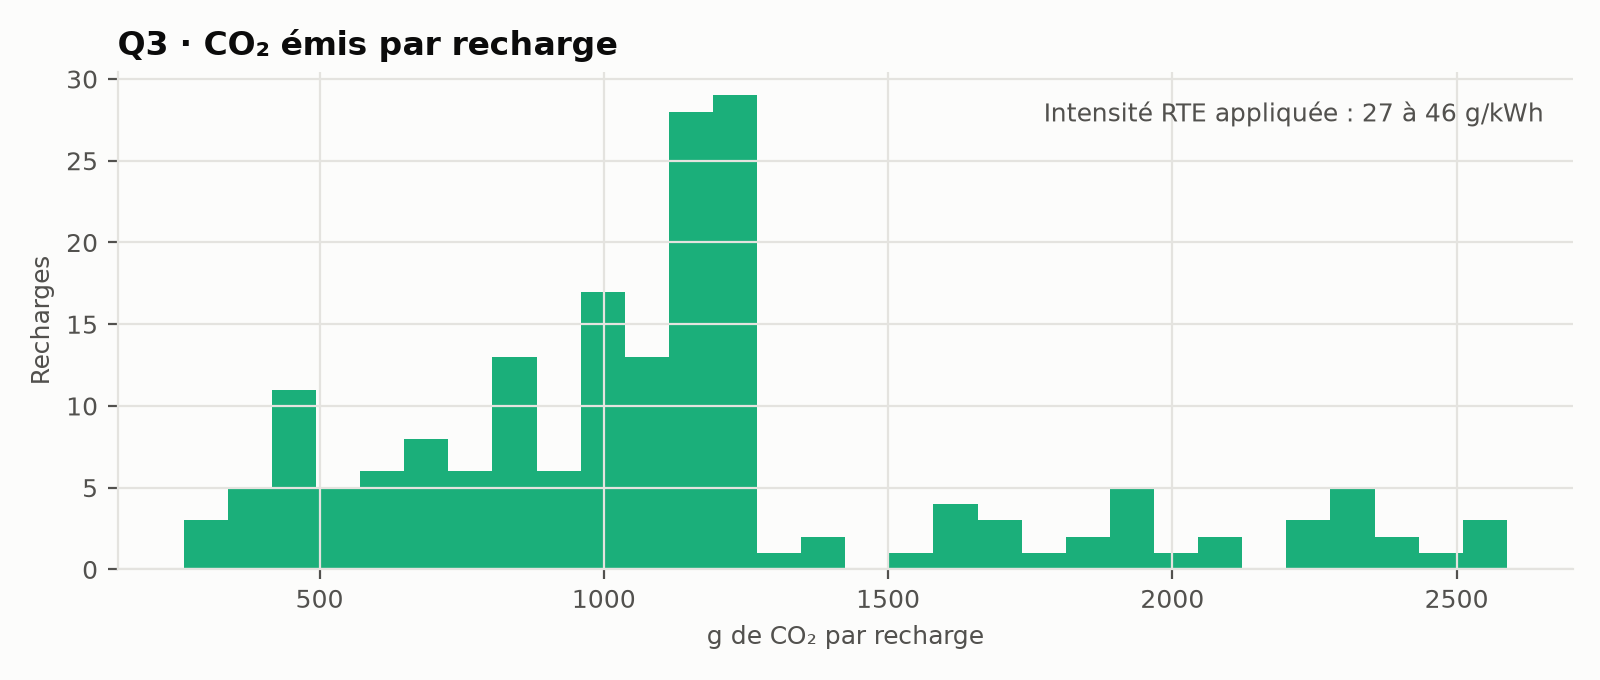
\includegraphics[width=0.86\linewidth]{q3_co2_par_recharge.png}
\end{figure}
186 recharges ont délivré 4,8~MWh et émis 211~kg de CO\textsubscript{2}, à l'intensité réelle du réseau ce soir-là (44~g/kWh en moyenne) :
1,1~kg par recharge en médiane. Le même calcul est affiché en direct pour chaque recharge en cours.

\subsection*{Q4 · Panne, rattrapage et charge}
\begin{figure}[H]
\centering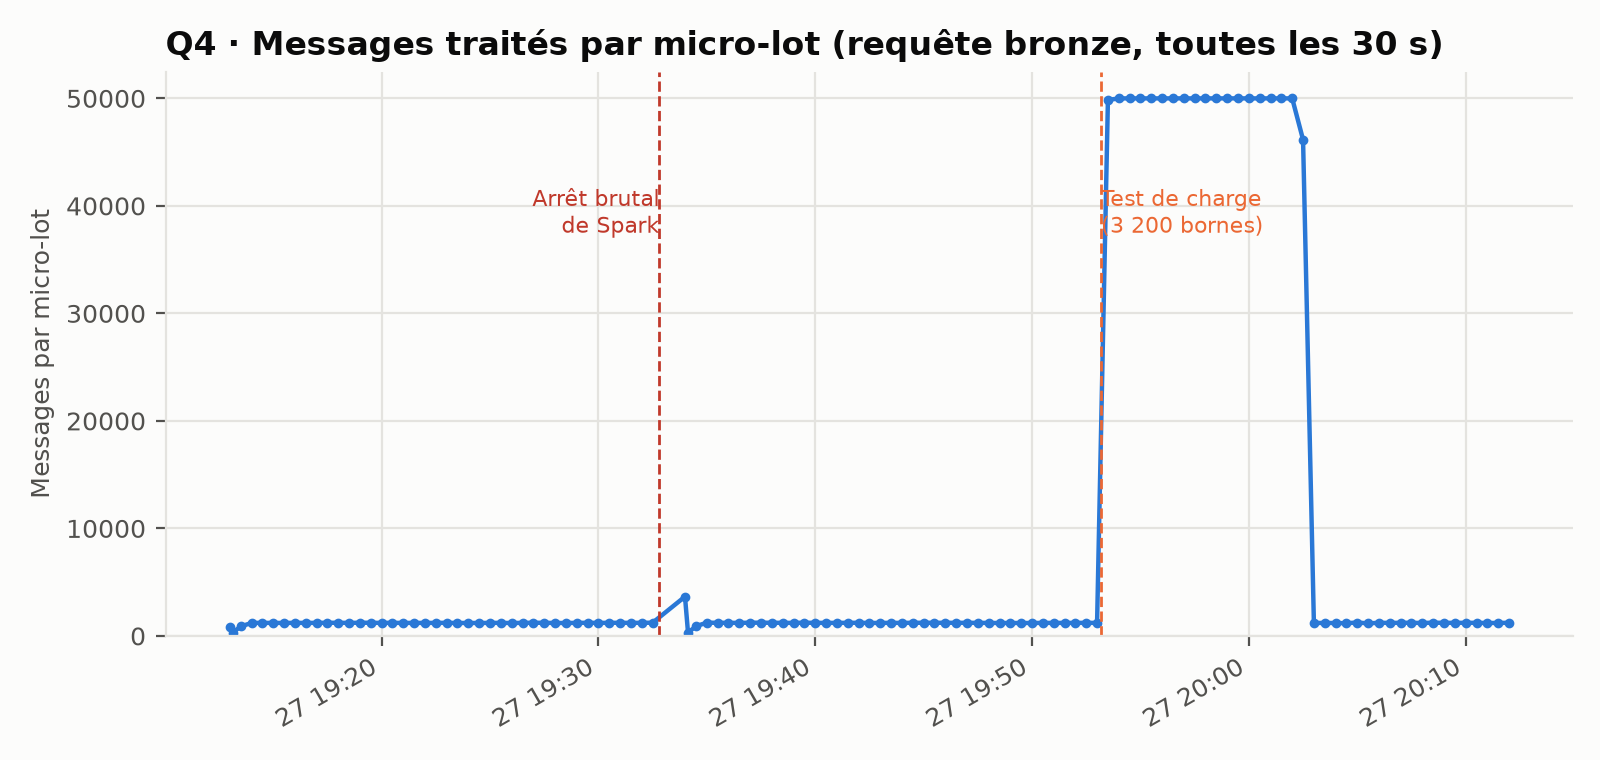
\includegraphics[width=0.86\linewidth]{q4_debit_reprise_charge.png}
\end{figure}

\begin{table}[H]
\centering\small
\begin{tabularx}{\linewidth}{@{}L{4.6cm} Y@{}}
\toprule
\textbf{Test de charge (≈ 2\,960 messages/s)} & \textbf{Résultat} \\
\midrule
Bronze et silver & Suivent : jusqu'à 5\,700 et 4\,600 messages/s \\
Moniteur à état & \textbf{Goulot d'étranglement} : ≈ 1\,440 messages/s ; détection à 130-160~s pendant la surcharge \\
Stabilité & Aucun plantage ; retard résorbé 10 minutes après la fin de la surcharge \\
Capacité & ≈ 7\,000 bornes à une mesure toutes les 5~s, pour un parc de 1\,200 \\
\bottomrule
\end{tabularx}
\caption{Ce que la plateforme tient sur un poste}
\end{table}

% =============================================================================
\section{Retour d'expérience}
\begin{table}[H]
\centering\small
\begin{tabularx}{\linewidth}{@{}L{4.3cm} Y@{}}
\toprule
\textbf{Défaut ou incident} & \textbf{Leçon} \\
\midrule
Les tests Spark étaient ignorés sans le dire & Un test « ignoré » n'est pas un test réussi : vérifier le nombre de tests exécutés \\
Colonne de dates vide refusée par Arrow & Le premier lot réel contient des cas qu'aucun exemple ne contenait \\
\texttt{event\_id} répétés après un redémarrage & Une clé de dédoublonnage doit être unique \textbf{dans le temps}, pas dans une exécution \\
Rapprochement faux au premier essai & Deux tables écrites par deux requêtes ne sont jamais au même instant : comparer un ensemble fixe \\
Bornes muettes manquées au rattrapage & Un délai en temps de traitement n'a pas de sens quand le temps est « accéléré » \\
Arrêts de Spark après mise en veille & Les checkpoints et la politique de redémarrage ont repris seuls ; un \texttt{docker kill} manuel, non \\
\bottomrule
\end{tabularx}
\caption{Ce que ce projet a appris}
\end{table}

% =============================================================================
\section{Feuille de route}
\begin{enumerate}[leftmargin=1.4em]
  \item \textbf{Capacité} : moniteur en Scala (\texttt{transformWithState}) ou cluster Dataproc, plus de partitions Kafka.
  \item \textbf{Alertes sortantes} : consommateur de \texttt{charger.alerts} vers SMS et ticketing, avec dédoublonnage.
  \item \textbf{Déploiement GCP} : \texttt{terraform plan} avec la DSI, puis Dataproc Serverless et Kafka managé.
  \item \textbf{Vraies bornes} : passerelle OCPP vers le topic \texttt{charger.telemetry}, sans changer le traitement.
\end{enumerate}

\end{document}
